\documentclass[tikz]{standalone}
\usepackage{fontspec}
\renewcommand*{\familydefault}{\sfdefault}
\usepackage{standalone}
\usepackage{amssymb}
\usetikzlibrary{decorations}
%\usetikzlibrary{arrows.meta, decorations.pathmorphing, decorations.pathreplacing, shapes.geometric}
\usetikzlibrary{bayesnet}

\begin{document}
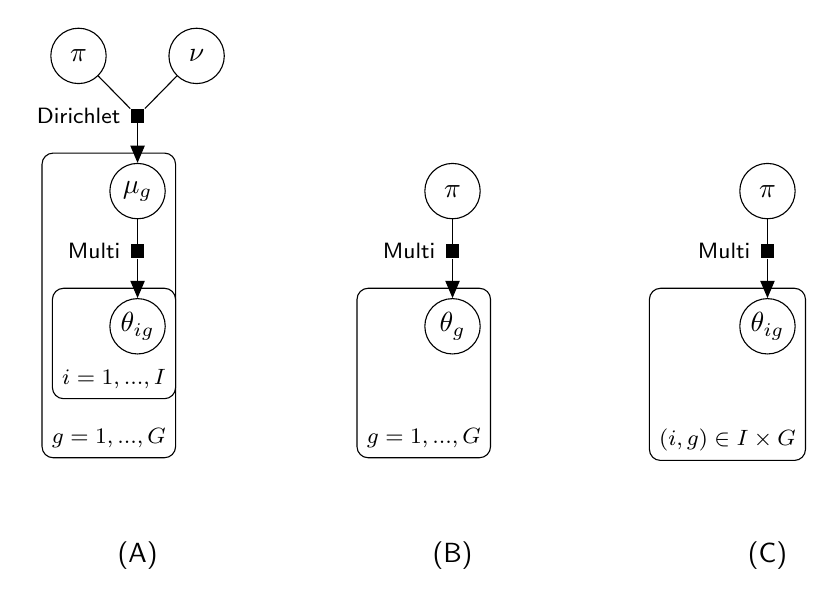
\begin{tikzpicture}%[font=\footnotesize, xscale=1.5]

\node[latent] (theta) {\(\theta_{ig}\)};
\factor[above=0.5 of theta, label=left:Multi]       {theta-f} {} {} {}; %
\node[latent, above=1.0 of theta] (mu) {\(\mu_g\)};
\factoredge {mu} {theta-f} {theta};

\factor[above=0.5 of mu, label=left:Dirichlet]       {mu-f} {} {} {}; %
\node[latent, above=1.0 of mu, xshift=-0.75 cm] (pi) {\(\pi\)};
\node[latent, above=1.0 of mu, xshift=0.75 cm] (nu) {\(\nu\)};
\factoredge {pi, nu} {mu-f} {mu};

\plate {i-p} {(theta)} {\(i=1,...,I\)} ;
\coordinate[below=0.75 of theta] (g-p-bottom) ;
\plate {g-p} {(theta) (mu) (g-p-bottom)} {\(g=1,...,G\)} ;

\node[below=1.5 of g-p-bottom] {(A)};


\begin{scope}[xshift=4 cm]

\node[latent] (theta-1) {\(\theta_{g}\)};
\factor[above=0.5 of theta-1, label=left:Multi]       {theta-f-1} {} {} {}; %
\node[latent, above=1.0 of theta-1] (pi-1) {\(\pi\)};
\factoredge {pi-1} {theta-f-1} {theta-1};

\coordinate[below=0.75 of theta-1] (g-p-bottom-1) ;
\plate {g-p-1} {(theta-1) (g-p-bottom-1)} {\(g=1,...,G\)} ;

\node[below=1.5 of g-p-bottom-1] {(B)};


\end{scope}

\begin{scope}[xshift=8 cm]

\node[latent] (theta-2) {\(\theta_{ig}\)};
\factor[above=0.5 of theta-2, label=left:Multi]       {theta-f-2} {} {} {}; %
\node[latent, above=1.0 of theta-2] (pi-2) {\(\pi\)};
\factoredge {pi-2} {theta-f-2} {theta-2};

\coordinate[below=0.75 of theta-2] (g-p-bottom-2) ;
\plate {g-p-2} {(theta-2) (g-p-bottom-2)} {\((i,g)\in I\times G\)} ;

\node[below=1.5 of g-p-bottom-2]  {(C)};


\end{scope}
\end{tikzpicture}
\end{document}
